\newcommand{\qm}{Quantenmechanik}

\section{Teilversuch 1: Lebensdauer eines Teilchen im unendlich tiefen Potientialtopf}
	\subsection{Teilversuch 1a: Verständnis zur Software SpektrumSLC.exe}
		\begin{figure}[!ht]
		    \centering
		    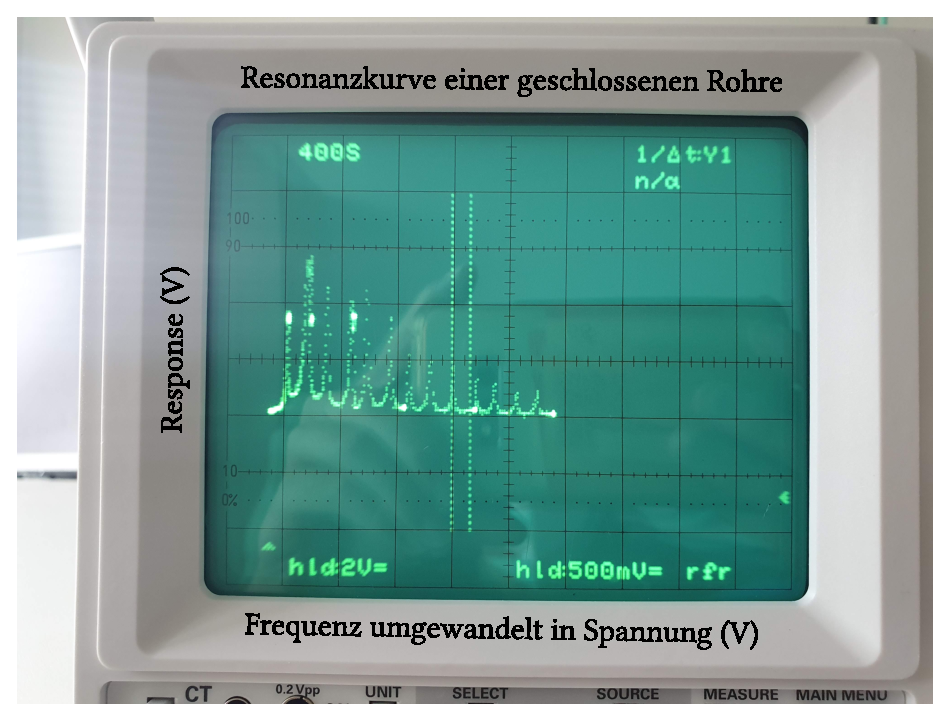
\includegraphics[width=0.8\textwidth]{./images/tv1a.eps}
		    \caption{Resonanzkurve einer geschlossenen Rohre ($d = \SI{225(1)}{\milli\meter}$)}
		    \label{fig:tv1a-osz}
		\end{figure}
		Diese Resonanzkurve ist auch was theoretisch zu erwarten ist. Da die Rohre geschlossen ist, kann nur stehende Wellen von bestimmten Frequenzen/Wellenlängen entstehen. Bei diesen stehenden Wellen erhalten wir dann ein Maxima für den Response. Somit ergibt sich eine Resonanzkurve mit mehrerer Peaks. 

		Die Beschreibung der Verarbeitungsschritte des Signals finden Sie im Laborprotokoll.

	\subsection{Teilversuch 1b: Messung der Lebensdauer eines Teilchen im unendlich tiefen Potientialtopf}
		Da die Fit Paramters nicht ausgedruckt sind, sind sie hier beschrieben:
		\begin{center}
			\begin{tabular}{l | *{4}{r}}
				\toprule
				Peak & \num{1} & \num{2} & \num{3} & \num{4} \\
				\midrule
				Frequency / \si{\hertz} & \num{5719.715} & \num{6853.203} & \num{7989.781} & \num{9124.208} \\
				Amplitude / a.u.        & \num{59.0441} & \num{41.929} & \num{31.0203} & \num{22.639} \\
				Width / \si{\hertz}     & \num{17.634} & \num{18.732} & \num{19.371} & \num{20.437} \\
				Phase / \si{\degree}    & \num{-46.7} & \num{-1.7} & \num{29.9} & \num{57.9} \\
				\bottomrule
				\toprule
				Peak & \num{5} & \num{6} & \num{7} & \num{8} \\
				\midrule
				Frequency / \si{\hertz} & \num{10259.772} & \num{11393.832} & \num{12524.178} & \num{13641.917} \\
				Amplitude / a.u.        & \num{14.1618} & \num{13.2206} & \num{9.5492} & \num{7.4138} \\
				Width / \si{\hertz}     & \num{22.807} & \num{23.386} & \num{27.648} & \num{33.978} \\
				Phase / \si{\degree}    & \num{63.8} & \num{90.7} & \num{98.3} & \num{133.8} \\
				\bottomrule
			\end{tabular}
		\end{center}
		Siehe Laborprotokoll für den Plot. Die Kurveanpassung sieht nach Augenmaß ziemlich gut aus. 

		\subsubsection{Regelmäßiger Abstand}
			Wie im letzten Teilversuch beschrieben, entstehen wegen der bestimmten Länge der Rohre nur bei bestimmen Wellenlänge stehende Wellen. Da die Rohre am beiden Enden geschlossen ist, muss die Schallgeschwindigkeit am Randen null sein, was zu einer Maxima im Druck führt. Diesen Druck messen wir dann mit unsere Mikrofon. Solche stehenede Wellen können wir mit Abbildung 1 der Anleitung veranschaulich machen:
			\begin{figure}[!ht]
			    \centering
			    \includegraphics[width=0.45\textwidth]{./images/standing-waves.jpg}
			    \caption{Stehende Welle bzw. stationäre Zustände in der Rohre/Potentialtopf}
			    \label{fig:standing-waves}
			    \vspace{-1em}
			\end{figure}

			Im Fall der Quantenmechanik muss die Aufenthaltswahrscheinkeit bei der Rände null sein, sind also hier als Minima der Wellenfunktion repräsentiert. 

			Im Fall der Akustische Resonanz sind jedoch die Ende bei einem Maximum und nicht Minimium, wie in der obigen Abbildung. Wir transformieren somit die Sinuskurven hier in Kosinuskurven, sodass am Ende Maxima sind.

			Die Randbedingung für eine stehende Welle ($\cong$ stationäre Zustand) bleibt unverändert:  
			\begin{align}
				L = \frac{n\lambda}{2} = \frac{nv}{2f} &&\Rightarrow&& f = \frac{v}{2L} \times n
			\end{align}
			Da hier der Fokus dieses Teilversuchs nicht die stehende Welle ist, sondern die Lebensdauer, machen wir nur eine grobe Abschätzung, ob die Ergenisse vernünftig sind. 

			Die Schallgeschwindigkeit im Luft beträgt ungefähr \SI{343}{\meter\per\second} bei \SI{20}{\celsius}\footnote{\url{https://www.weather.gov/epz/wxcalc_speedofsound}, \today}. Man soll also $f$ in Vielfaches von 
			\begin{align}
				\frac{v}{2L} = \frac{\SI{343}{\meter\per\second}}{2\left(\SI{0.15}{\meter}\right)} = \SI{1143}{\hertz}
			\end{align}
			erhalten.
			\begin{center}
				\begin{tabular}{l *{7}{r}}
					\toprule
					Peak $i \rightarrow j$ & \num{1} $\rightarrow$ \num{2} & \num{2} $\rightarrow$ \num{3} & \num{3} $\rightarrow$ \num{4} & \num{4} $\rightarrow$ \num{5} & \num{5} $\rightarrow$ \num{6} & \num{6} $\rightarrow$ \num{7} & \num{7} $\rightarrow$ \num{8} \\
					\midrule
					$f_j - f_i$ / \si{\hertz} & \num{1133.488} & \num{1136.578} & \num{1134.427} & \num{1135.564} & \num{1134.06} & \num{1130.346} & \num{1117.739} \\
					\bottomrule
				\end{tabular}
			\end{center}
			Wir plotten nun die Frequenz $f$ gegen die Peak-Nummer $n$ und führen eine Kurveanpassung zu $f = mn + c$ durch (Siehe Appendix \ref{appdx:tv1-1}):
			\begin{figure}[!ht]
			    \centering
			    % GNUPLOT: LaTeX picture with Postscript
\begingroup
  \makeatletter
  \providecommand\color[2][]{%
    \GenericError{(gnuplot) \space\space\space\@spaces}{%
      Package color not loaded in conjunction with
      terminal option `colourtext'%
    }{See the gnuplot documentation for explanation.%
    }{Either use 'blacktext' in gnuplot or load the package
      color.sty in LaTeX.}%
    \renewcommand\color[2][]{}%
  }%
  \providecommand\includegraphics[2][]{%
    \GenericError{(gnuplot) \space\space\space\@spaces}{%
      Package graphicx or graphics not loaded%
    }{See the gnuplot documentation for explanation.%
    }{The gnuplot epslatex terminal needs graphicx.sty or graphics.sty.}%
    \renewcommand\includegraphics[2][]{}%
  }%
  \providecommand\rotatebox[2]{#2}%
  \@ifundefined{ifGPcolor}{%
    \newif\ifGPcolor
    \GPcolortrue
  }{}%
  \@ifundefined{ifGPblacktext}{%
    \newif\ifGPblacktext
    \GPblacktexttrue
  }{}%
  % define a \g@addto@macro without @ in the name:
  \let\gplgaddtomacro\g@addto@macro
  % define empty templates for all commands taking text:
  \gdef\gplbacktext{}%
  \gdef\gplfronttext{}%
  \makeatother
  \ifGPblacktext
    % no textcolor at all
    \def\colorrgb#1{}%
    \def\colorgray#1{}%
  \else
    % gray or color?
    \ifGPcolor
      \def\colorrgb#1{\color[rgb]{#1}}%
      \def\colorgray#1{\color[gray]{#1}}%
      \expandafter\def\csname LTw\endcsname{\color{white}}%
      \expandafter\def\csname LTb\endcsname{\color{black}}%
      \expandafter\def\csname LTa\endcsname{\color{black}}%
      \expandafter\def\csname LT0\endcsname{\color[rgb]{1,0,0}}%
      \expandafter\def\csname LT1\endcsname{\color[rgb]{0,1,0}}%
      \expandafter\def\csname LT2\endcsname{\color[rgb]{0,0,1}}%
      \expandafter\def\csname LT3\endcsname{\color[rgb]{1,0,1}}%
      \expandafter\def\csname LT4\endcsname{\color[rgb]{0,1,1}}%
      \expandafter\def\csname LT5\endcsname{\color[rgb]{1,1,0}}%
      \expandafter\def\csname LT6\endcsname{\color[rgb]{0,0,0}}%
      \expandafter\def\csname LT7\endcsname{\color[rgb]{1,0.3,0}}%
      \expandafter\def\csname LT8\endcsname{\color[rgb]{0.5,0.5,0.5}}%
    \else
      % gray
      \def\colorrgb#1{\color{black}}%
      \def\colorgray#1{\color[gray]{#1}}%
      \expandafter\def\csname LTw\endcsname{\color{white}}%
      \expandafter\def\csname LTb\endcsname{\color{black}}%
      \expandafter\def\csname LTa\endcsname{\color{black}}%
      \expandafter\def\csname LT0\endcsname{\color{black}}%
      \expandafter\def\csname LT1\endcsname{\color{black}}%
      \expandafter\def\csname LT2\endcsname{\color{black}}%
      \expandafter\def\csname LT3\endcsname{\color{black}}%
      \expandafter\def\csname LT4\endcsname{\color{black}}%
      \expandafter\def\csname LT5\endcsname{\color{black}}%
      \expandafter\def\csname LT6\endcsname{\color{black}}%
      \expandafter\def\csname LT7\endcsname{\color{black}}%
      \expandafter\def\csname LT8\endcsname{\color{black}}%
    \fi
  \fi
    \setlength{\unitlength}{0.0500bp}%
    \ifx\gptboxheight\undefined%
      \newlength{\gptboxheight}%
      \newlength{\gptboxwidth}%
      \newsavebox{\gptboxtext}%
    \fi%
    \setlength{\fboxrule}{0.5pt}%
    \setlength{\fboxsep}{1pt}%
    \definecolor{tbcol}{rgb}{1,1,1}%
\begin{picture}(8640.00,5760.00)%
    \gplgaddtomacro\gplbacktext{%
      \csname LTb\endcsname%%
      \put(1078,704){\makebox(0,0)[r]{\strut{}$4000$}}%
      \put(1078,1437){\makebox(0,0)[r]{\strut{}$6000$}}%
      \put(1078,2169){\makebox(0,0)[r]{\strut{}$8000$}}%
      \put(1078,2902){\makebox(0,0)[r]{\strut{}$10000$}}%
      \put(1078,3634){\makebox(0,0)[r]{\strut{}$12000$}}%
      \put(1078,4367){\makebox(0,0)[r]{\strut{}$14000$}}%
      \put(1078,5099){\makebox(0,0)[r]{\strut{}$16000$}}%
      \put(1210,484){\makebox(0,0){\strut{}$0$}}%
      \put(1991,484){\makebox(0,0){\strut{}$1$}}%
      \put(2773,484){\makebox(0,0){\strut{}$2$}}%
      \put(3554,484){\makebox(0,0){\strut{}$3$}}%
      \put(4336,484){\makebox(0,0){\strut{}$4$}}%
      \put(5117,484){\makebox(0,0){\strut{}$5$}}%
      \put(5899,484){\makebox(0,0){\strut{}$6$}}%
      \put(6680,484){\makebox(0,0){\strut{}$7$}}%
      \put(7462,484){\makebox(0,0){\strut{}$8$}}%
      \put(8243,484){\makebox(0,0){\strut{}$9$}}%
    }%
    \gplgaddtomacro\gplfronttext{%
      \csname LTb\endcsname%%
      \put(209,2901){\rotatebox{-270}{\makebox(0,0){\strut{}Eigenfrequenz $f$ ($\si{\hertz}$)}}}%
      \put(4726,154){\makebox(0,0){\strut{}Peak-Nummer $n$ (Einheitlos)}}%
      \csname LTb\endcsname%%
      \put(7256,1427){\makebox(0,0)[r]{\strut{}$(1132,83340)n + (4590,57543)$}}%
      \csname LTb\endcsname%%
      \put(7256,987){\makebox(0,0)[r]{\strut{}Messpunkte}}%
      \csname LTb\endcsname%%
      \put(4726,5429){\makebox(0,0){\strut{}Eigenfrequenz $f$ gegen Peak-Nummer $n$}}%
    }%
    \gplbacktext
    \put(0,0){\includegraphics[width={432.00bp},height={288.00bp}]{tv1-1}}%
    \gplfronttext
  \end{picture}%
\endgroup

			    \caption{Kurveanpassung: \texttt{rms of residuals} $=\num{6.26596}$, klein gegenüber Messwerten}
			    \label{fig:tv1-1}
			\end{figure}

			Als Endergebnis erhalten wir $m = \SI{1132.8(10)}{\hertz}$.

			% Wir erhalten also $\overline{f_j - f_i} = \SI{1131.7(25)}{\hertz}$, wobei den Mittelwert mittels \texttt{AVERAGE} und Unsicherheit mittels $\nicefrac{\text{\texttt{STDEV.S}}}{\sqrt{N}}$ berechnet war. 

			Diese zwei Ergebnisse unterscheidet sich zwar signifikant voneinander, ist aber Großeordnungsmäßig ziemlich nah. Die Abweichung ist wahrscheinlich wegen der nicht genauen Temperatur. Außerdem ist der letzte Abstand von \SI{1117.739}{\hertz} ziemlich weit von der anderen Werten. Die Randbedingungen entsprechen vielleicht nicht die Echten im Experiment.

		\subsubsection{Abnehmende Amplitude}
			Man sieht auch vom Plot im Laborprotokoll, dass die Amplitude mit steigenden $n$ abnimmt. Das ist Analog zu den abnehmenden Koeffizienten der Fouriertransformation im Quantenmechanischen Fall.

		\subsubsection{Energieniveau}
			Die horizontale $f$-Achse stellt mit der Resonanzpeaks eine Quantisierung dar. Die Achse kann also für die quantisierte Energieniveau dienen.

		\subsubsection{Lebensdauer}
			In der Akustik is die Lebensdauer von Reibung bedingt. Die Frequenzen kann man auch nicht direkt in Energie umwandeln. Die Resonanzen sind eine Folge der gedämpfte angetriebene Schwingung, somit bleibt auch eine stehende Welle entstehen, wenn sie vom Lautsprecher weiter angetrieben ist, egal welche Frequenz sie ist. 

			In der \qm{} geht es um einen statistischen Prozess und kommt aus der Heisenbergischen Unschärferelation. Ein angeregter Zustand zerfällt in endlicher Zeit in den Grundzustand und die Lebensdauer beschreibt die mittlere Zeit, in der der angeregete Zustand angeregt bleibt. Das kann man leider nicht im akustischen Fall nachmachen.

			Aus der Heisenbergischen Unschärferelation ist $\Delta E \Delta t \geq \nicefrac{h}{2\pi}$. Da $\Delta E \propto \Delta f$ ist, ist die Lebensdauer $\Delta t$ somit propotional zu $\nicefrac{1}{\Delta f}$. Wir bringen diese Analogie zu Akustik und plotten nun $\nicefrac{1}{\Delta f}$ gegen $n$ und führe eine Kurveanpassung durch:
			\begin{figure}[!ht]
			    \centering
			    \vspace{-1em}
			    % https://tex.stackexchange.com/a/98142
			    \resizebox{.9\textwidth}{!}{% GNUPLOT: LaTeX picture with Postscript
\begingroup
  \makeatletter
  \providecommand\color[2][]{%
    \GenericError{(gnuplot) \space\space\space\@spaces}{%
      Package color not loaded in conjunction with
      terminal option `colourtext'%
    }{See the gnuplot documentation for explanation.%
    }{Either use 'blacktext' in gnuplot or load the package
      color.sty in LaTeX.}%
    \renewcommand\color[2][]{}%
  }%
  \providecommand\includegraphics[2][]{%
    \GenericError{(gnuplot) \space\space\space\@spaces}{%
      Package graphicx or graphics not loaded%
    }{See the gnuplot documentation for explanation.%
    }{The gnuplot epslatex terminal needs graphicx.sty or graphics.sty.}%
    \renewcommand\includegraphics[2][]{}%
  }%
  \providecommand\rotatebox[2]{#2}%
  \@ifundefined{ifGPcolor}{%
    \newif\ifGPcolor
    \GPcolortrue
  }{}%
  \@ifundefined{ifGPblacktext}{%
    \newif\ifGPblacktext
    \GPblacktexttrue
  }{}%
  % define a \g@addto@macro without @ in the name:
  \let\gplgaddtomacro\g@addto@macro
  % define empty templates for all commands taking text:
  \gdef\gplbacktext{}%
  \gdef\gplfronttext{}%
  \makeatother
  \ifGPblacktext
    % no textcolor at all
    \def\colorrgb#1{}%
    \def\colorgray#1{}%
  \else
    % gray or color?
    \ifGPcolor
      \def\colorrgb#1{\color[rgb]{#1}}%
      \def\colorgray#1{\color[gray]{#1}}%
      \expandafter\def\csname LTw\endcsname{\color{white}}%
      \expandafter\def\csname LTb\endcsname{\color{black}}%
      \expandafter\def\csname LTa\endcsname{\color{black}}%
      \expandafter\def\csname LT0\endcsname{\color[rgb]{1,0,0}}%
      \expandafter\def\csname LT1\endcsname{\color[rgb]{0,1,0}}%
      \expandafter\def\csname LT2\endcsname{\color[rgb]{0,0,1}}%
      \expandafter\def\csname LT3\endcsname{\color[rgb]{1,0,1}}%
      \expandafter\def\csname LT4\endcsname{\color[rgb]{0,1,1}}%
      \expandafter\def\csname LT5\endcsname{\color[rgb]{1,1,0}}%
      \expandafter\def\csname LT6\endcsname{\color[rgb]{0,0,0}}%
      \expandafter\def\csname LT7\endcsname{\color[rgb]{1,0.3,0}}%
      \expandafter\def\csname LT8\endcsname{\color[rgb]{0.5,0.5,0.5}}%
    \else
      % gray
      \def\colorrgb#1{\color{black}}%
      \def\colorgray#1{\color[gray]{#1}}%
      \expandafter\def\csname LTw\endcsname{\color{white}}%
      \expandafter\def\csname LTb\endcsname{\color{black}}%
      \expandafter\def\csname LTa\endcsname{\color{black}}%
      \expandafter\def\csname LT0\endcsname{\color{black}}%
      \expandafter\def\csname LT1\endcsname{\color{black}}%
      \expandafter\def\csname LT2\endcsname{\color{black}}%
      \expandafter\def\csname LT3\endcsname{\color{black}}%
      \expandafter\def\csname LT4\endcsname{\color{black}}%
      \expandafter\def\csname LT5\endcsname{\color{black}}%
      \expandafter\def\csname LT6\endcsname{\color{black}}%
      \expandafter\def\csname LT7\endcsname{\color{black}}%
      \expandafter\def\csname LT8\endcsname{\color{black}}%
    \fi
  \fi
    \setlength{\unitlength}{0.0500bp}%
    \ifx\gptboxheight\undefined%
      \newlength{\gptboxheight}%
      \newlength{\gptboxwidth}%
      \newsavebox{\gptboxtext}%
    \fi%
    \setlength{\fboxrule}{0.5pt}%
    \setlength{\fboxsep}{1pt}%
    \definecolor{tbcol}{rgb}{1,1,1}%
\begin{picture}(7200.00,4320.00)%
    \gplgaddtomacro\gplbacktext{%
      \csname LTb\endcsname%%
      \put(1078,704){\makebox(0,0)[r]{\strut{}$0,02$}}%
      \put(1078,1073){\makebox(0,0)[r]{\strut{}$0,025$}}%
      \put(1078,1443){\makebox(0,0)[r]{\strut{}$0,03$}}%
      \put(1078,1812){\makebox(0,0)[r]{\strut{}$0,035$}}%
      \put(1078,2182){\makebox(0,0)[r]{\strut{}$0,04$}}%
      \put(1078,2551){\makebox(0,0)[r]{\strut{}$0,045$}}%
      \put(1078,2920){\makebox(0,0)[r]{\strut{}$0,05$}}%
      \put(1078,3290){\makebox(0,0)[r]{\strut{}$0,055$}}%
      \put(1078,3659){\makebox(0,0)[r]{\strut{}$0,06$}}%
      \put(1210,484){\makebox(0,0){\strut{}$0$}}%
      \put(1831,484){\makebox(0,0){\strut{}$1$}}%
      \put(2453,484){\makebox(0,0){\strut{}$2$}}%
      \put(3074,484){\makebox(0,0){\strut{}$3$}}%
      \put(3696,484){\makebox(0,0){\strut{}$4$}}%
      \put(4317,484){\makebox(0,0){\strut{}$5$}}%
      \put(4939,484){\makebox(0,0){\strut{}$6$}}%
      \put(5560,484){\makebox(0,0){\strut{}$7$}}%
      \put(6182,484){\makebox(0,0){\strut{}$8$}}%
      \put(6803,484){\makebox(0,0){\strut{}$9$}}%
    }%
    \gplgaddtomacro\gplfronttext{%
      \csname LTb\endcsname%%
      \put(209,2181){\rotatebox{-270}{\makebox(0,0){\strut{}Lebensdauer $\nicefrac{1}{\Delta f}$ ($\si{\second}$)}}}%
      \put(4006,154){\makebox(0,0){\strut{}Peak-Nummer $n$ (Einheitlos)}}%
      \csname LTb\endcsname%%
      \put(5816,3486){\makebox(0,0)[r]{\strut{}$(-0,0003245)x^2 + (-0,0007549)x + (0,0570273)$}}%
      \csname LTb\endcsname%%
      \put(5816,3266){\makebox(0,0)[r]{\strut{}Messpunkte}}%
      \csname LTb\endcsname%%
      \put(4006,3989){\makebox(0,0){\strut{}Lebensdauer $\nicefrac{1}{\Delta f}$ gegen Peak-Nummer $n$}}%
    }%
    \gplbacktext
    \put(0,0){\includegraphics[width={360.00bp},height={216.00bp}]{tv1-2}}%
    \gplfronttext
  \end{picture}%
\endgroup
}
			    \caption{Lebensdauer in Abhängigkeit von Peak-Nummer, \texttt{rms of residuals} $=\num{0.00122663}$, klein gegenüber Messwerten}
			    \label{fig:tv1-2}
			    \vspace{-1em}
			\end{figure}
			
			Man erkennt hier einen abnehmenden Trend mit steigender Peak-Nummer $n$. Aus der Anleitung ist die Energie $\Gamma = \nicefrac{\hbar}{\tau}$ im quantenmechanischen Fall mit der Lebensdauer verbunden. Also gilt:
			\begin{align}
				\tau = \frac{\hbar}{\Gamma} &&\Rightarrow&& E_n \propto -\frac{1}{n^2} &&\Rightarrow&& \tau \propto n^2
			\end{align}
			Mit steigende Energie soll man dann eine kleinere Lebensdauer erwarten. Das ist auch genau das, was wir hier beobachten können. Die Fehlerbalken werden auch nicht berücksichtigt, weil dies vom Fit-Software nicht gegeben ist. Die Kurveanpassung, sofern sinnvoll, sieht auch gut aus. 

			Es ist hier eine Kurveanpassung zu einer quadratischen Funktion (QM) durchgeführt, weil ich keine Theorie zur Abhängigkeit der Lebensdauer mit der Peak-Nummer in der Anleitung oder im Internet gefunden. Wenn solche Abhängigkeit tatsächlich existiert, werde ich mich freuen, wenn wir sie im Nachgespräch klären können.











